Unfortunately, the SAR image that is created is not always clear or useful. To assess and increase the clarity and usefulness of the image, preprocessing is done. An overview of the process is presented in figure \ref{fig:overview}.
\begin{figure}[H]
	\centering
    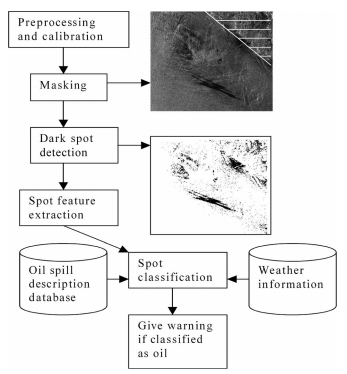
\includegraphics[width=50mm,scale=0.3]{./img/detection_diagram.png}
    \caption{\footnotesize{Overview for the oil spill detection approach \cite{Solberg200745}}}
    \label{fig:overview}
\end{figure}
First, there is a general quality assessment. If the image is blurred in general, it will be impossible to get any information out of it.
Afterwards, several preprocessing steps are executed to improve the contrast between dark spots and the water surrounding them, as well as flag certain dark spots to be ignored. 
It is important that experts look at noise removal. One of the most common versions of noise is speckle noise. Speckle noise is caused naturally by a disruption in the phase of radio waves. Radio waves leave the sensor all in the same phase. Once they interact with an object, they scatter and are out of phase with each other. If they interact with each other, the result will be a darker or lighter pixel than it should (e.g. oil will be lighter, water will be darker). Multi-look processing and spatial filtering are examples of techniques that can be done to reduce speckle noise \cite{simard1998analysis}.

Experts also flag (mask) areas in the image which might interfere with the classification process. These areas include shorelines, land and ships, as these would all be represented by dark areas in the images. Land masses are usually identified using GPS and marked with Geographical Information System \cite{star1990geographic}. These systems allow for the storing, analyzing and manipulation of maps and images using geographical information. Ships can be identified if their route or position is known. A problems arises when the information is not public or missing in some way.
Another possibility is that dark spots are caused by algae or seaweed infestations \cite{fingas2014review}. These can be masked if, for instance, local ecological groups have knowledge of these formations. Grease ice and rain cells are some more examples of what can be mistaken for oil spills \cite{Brekke200595}. The problem is that it is hard to filter out every dark spot, since there is so much information and some critical information might not be public or present.

These preprocessing steps will make classification easier, but is still a difficult task. In some cases, even a human expert cannot tell the difference \cite{Keramitsoglou2006640}. Through image segmentation, all dark spots are taken into isolation and the values of predefined features are extracted from them. This segmentation can be done manually but there have also been numerous proposals to do this with different algorithms \cite{ma2011sar,fjortoft1998optimal, ye2002wavelet} Classification can now be performed by using the features as input where the output of the chosen classifier will be the probability of the dark spot being an oil spill or a lookalike. 
High or low wind areas are also taken into consideration as they change the surface of the water and oil slicks. This can influence the reflection of radio waves and in turn the image \cite{fingas2014review}.

In an automated detection system, a high oil spill probability can lead to a warning message so that it can be further examined by an expert.


